% !TeX encoding=utf8
% !TeX spellcheck = en-US

\section{Advanced EaaS Services}
\label{sec:adv}

As depicted in \Cref{fig:arch}, the OC platform design follows a three-tier approach, addressing data provisioning, platform management, and experimentation support. The Site Tier accounts for the data sources (e.g., cities) federated in the OC platform (named OC site). The Platform Tier holds the platform services, which are exposed for experimentation in the Experimentation Tier. The persistence within the Platform Tier relies on Orion, which is  built around the NGSI~9/10 protocols. It manages entries, called assets, which can represent devices, places, buildings and any other context information entities (including virtual objects). Each asset holds a set of typed attributes which can be updated on the fly~\cite{gutierrez1}. The Platform Tier has been designed using loosely coupled and distributed components following the micro-service architecture pattern~\cite{newman2015building}. This allows tailored deployments involving only the mandatory, or baseline services, so that others (i.e., APIs, tools and portals) can be optionally deployed.

The rest of this section covers improvements performed in the Platform and Experimentation Tiers. This tier makes use of the EaaS APIs (see \Cref{fig:arch}), and it embraces tools and Web-based user interfaces (web portals). Each EaaS service (i.e., API, tool and portal) is implemented as a micro-service. In this sense, some of them are standalone applications, while others rely on baseline services, such as the Orion or the User Management. For a more detailed description of the platform, the reader may refer to ~\cite{gutierrez1}, which covers the EaaS services, which were used in the first open call. \highlighttext{Based on feedback from experimenters in the first open call, we re-factored and extended the OC services, and present these in the following sub-sections.}

\subsection{User Management}

Within OC, we cater to different stakeholder ``roles'', e.g., administrators, site managers, experimenters and participants. An administrator is the technical administrator of the OC platform and, therefore, has access to information of all experiments at platform level. A site manager manages an OC site, which is a set of assets under a common administrative domain available for experimentation, e.g., the assets of a city. Each role is allowed to access different systems, which consists of an API and a portal. To handle this, we developed a User Management system to handle authentication and authorization.

\begin{figure}
%	\todo[inline,author=Dennis]{Shall I create a blue version of the figure?}
    \centering 
	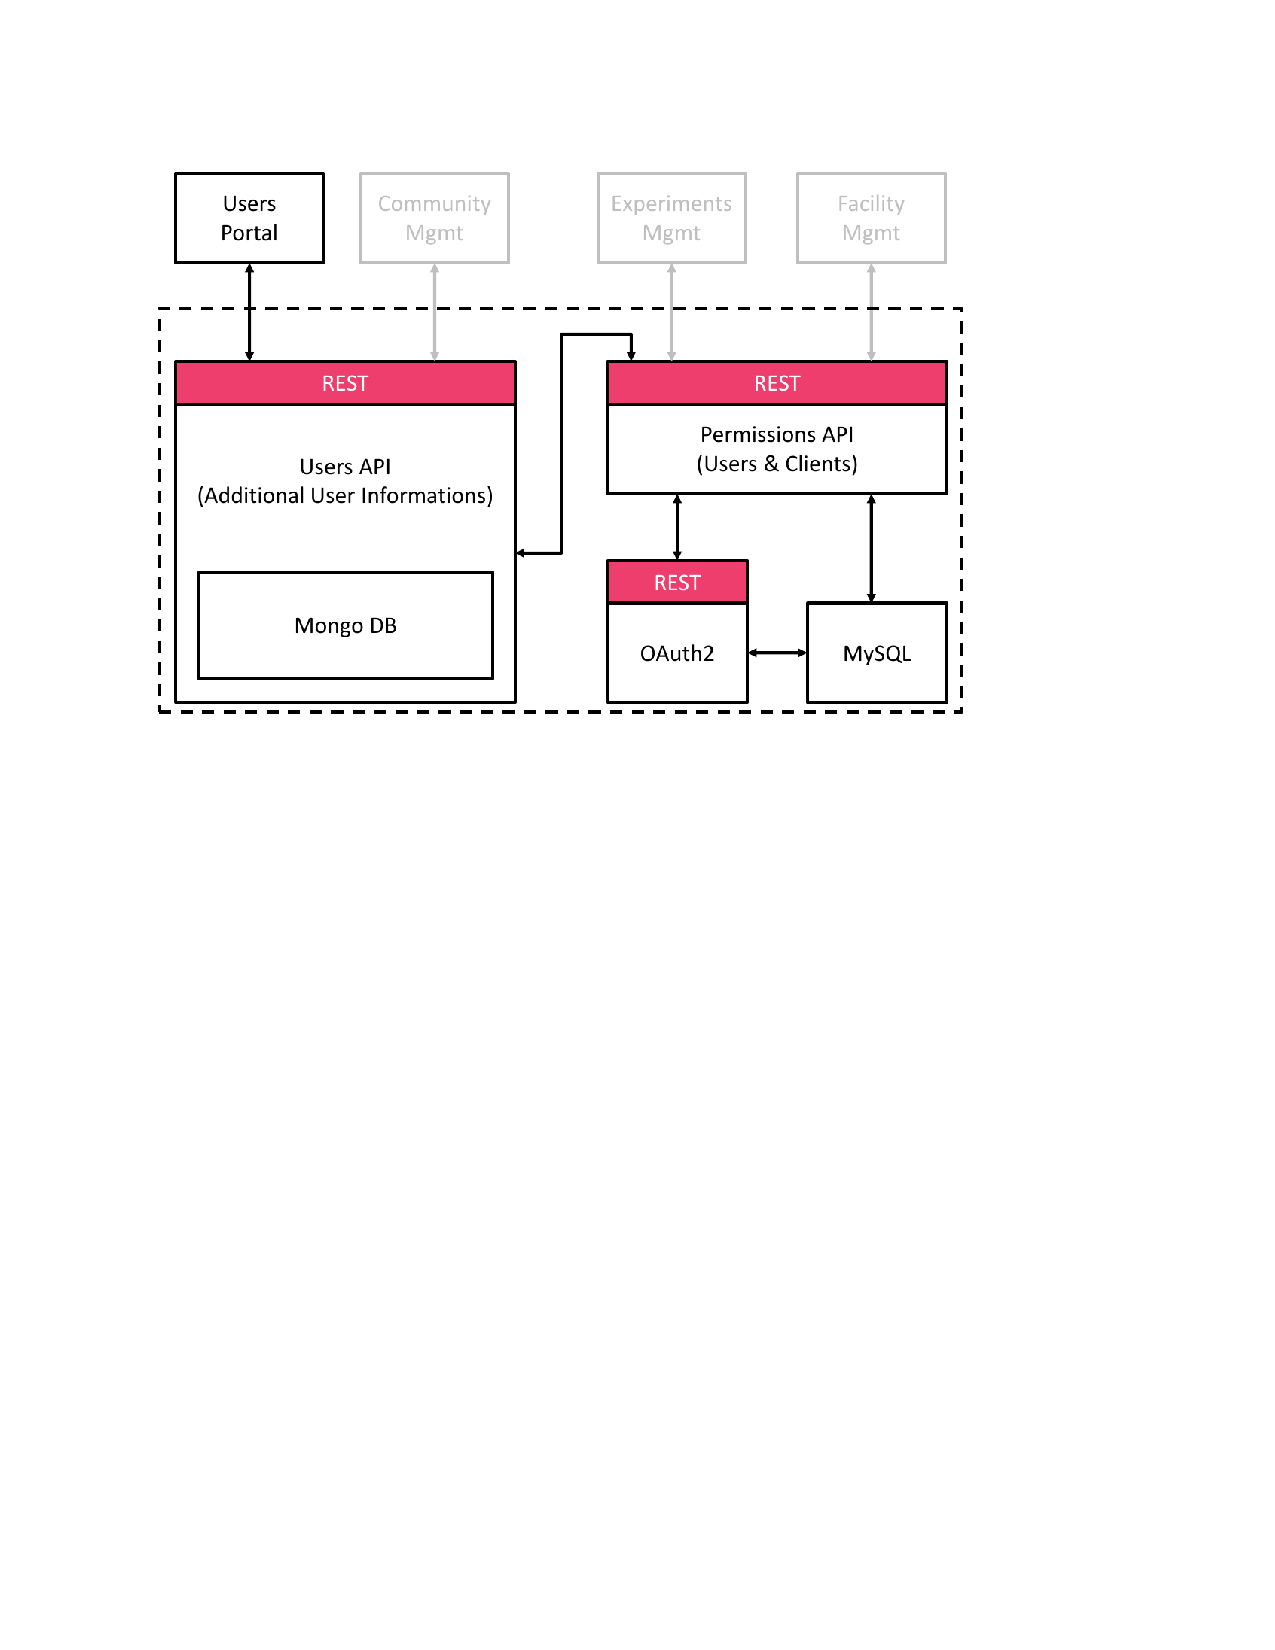
\includegraphics[scale = .5]{figures/user}
	\caption{User Management APIs}
	\label{fig:user}	
\end{figure}

The User Management API is based on OAuth2's API~\cite{rfc6749}, with a single sign-on service, a \emph{Users API}, and a \emph{Permissions API} (see \Cref{fig:user}). They are used to manage accounts for users and clients (e.g., OC services). We use KeyCloak\footnote{https://www.keycloak.org} as an OAuth2 server. %To manage accounts, it provides an HTTP-based RESTful API~\cite{fielding2000architectural}, which is only usable by KeyCloak-specific \emph{admin} accounts. 
To allow other OC services to manage accounts, we created the Permissions API, which acts as a configuration proxy for a more fine-grained access to the roles and permissions of accounts. Users must register at the server and verify their account by email. Afterwards, a user can log into all OC services by using a single account. %In case of the portals, a user needs to log in only once, since a session is used to remember the user. 

The \emph{Users Portal} allows users to manage their data, such as user and real names, nationality, email, age, etc. The Users API allows a quick and efficient user search for other OC services, since it uses MongoDB\footnote{https://www.mongodb.com}. Some information like the username, email and password is synced between the Users API and the KeyCloak server. Authentication and authorization are still handled by the OAuth2 API, the other OC services can use the Users API to manage accounts.

\subsection{Experiment Management}

One of the key aspects of the OC platform is the definition of an experimentation management system, able to fulfill the requirements of potentially heterogeneous experiments. This system has been implemented as a set of APIs exposed through three web portals. First, the \textit{Experimenter Portal} allows experimenters to manage all aspects related to experiment management and exploitation. Closely related, the \textit{Communities Portal} enables the grouping of users, based on their interests and preferences, into the so called communities. Finally, the \textit{Participant Portal} permits potential participants to manage the experiments in which they are enrolled. \highlighttext{We briefly describe the functionalities of each of the web portals in the following.}

\subsubsection{Participant Portal}

This portal is used by users registered in OC, who have stated their willingness to participate in experiments, and it offers three main functionalities:

\begin{itemize}
	\item\emph{Experiment search}: All public experiments are visible to the participants, they can proactively select those taking place close to them or that are considered interesting, according to the experiment information.
	\item\emph{Notifications}: Participants can be notified about any event happening in the experiments they are involved in, and they can be invited to new experiments. It is worth noting that all interactions happen in \textit{an anonymous way}. Experimenters are not aware of the identity of participants.
	\item\emph{Enrolling management}: Participants can decide to leave an experiment at any point. It is applied to both experiments, which they proactively joined, and those which they were invited in.
\end{itemize}

\subsubsection{Communities Portal}
 
Once users register in OC, they can complete their profile by providing more information about their interests and preferences. Through the Communities Portal, administrators and experimenters can filter users and create \emph{communities}. A community is a virtual group linked to an experimenter or administrator, in a way that users and participants are not aware of the communities they belong to. %In the same way, 
Moreover, experimenters and administrators are not aware of the actual identity of the user in their communities, but they see simple indicators on the characteristics of their community's audience.

\subsubsection{Experimenter Portal}

This portal is the entry point of experimenters to the OC platform, and serves as a hub for the experimentation services. Following the micro-service design of the entire OC platform, the Experimenter Portal incorporates new services as independent views which may eventually be deactivated depending on the actual requirements. \highlighttext{By using the Experimenter Portal, experimenters can perform the following tasks}:
%The main functionalities provided by the Experimenter Portal are related to the management of the experiment instance, and cover deployment and experimentation:

\begin{itemize}
	\item \emph{Creation and management of experiments}: This functionality utilizes the User Management API. \highlighttext{Following the dominant concept in IoT experimentation, each experiment instance is seen as a virtual testbed, and uniquely identified throughout the whole platform. This way experiment datasets and management information can be isolated. In addition, at any moment experiments can be stopped/restarted and edited (e.g., name, description, etc.)}. 
	\item \emph{Creation and management of assets}: Leveraging the public platform APIs, the Experimenter Portal provides a graphical UI to create and edit assets, in order for experimenters to become familiar with the data format. \highlighttext{In particular, the graphical UI is a JSON editor able to check that the data follows the OrganiCity format, providing useful warning messages otherwise.}
	\item \emph{Experiment team management}: \highlighttext{Since co-creative experiments usually involve development teams rather than a single person, the Experimenter Portal also permits editing such teams. In this regard, at any moment the creator of the experiment can edit the team by adding or removing their members.}
\end{itemize}	

Apart from the aforementioned functionalities, the Experimenter Portal also provides views closely related to other services, and that can be used by the experimenters.

\paragraph{Annotations}

The Experimenter Portal offers a UI to manage \emph{tags} that can be applied on the assets created under each experiment. Experimenters can both select tags provided by the OC platform itself, or define new ones, available only for their own experiment. Tags are explained in more detail in \Cref{sec:annotation-service}.

\paragraph{Participants Management and Engagement Monitoring}

By using the communities created with the Communities Portal, experimenters can invite people to their experiments, and check whether or not invitations have been accepted.
In addition, experimenters can define engagement metrics as a function taking into account different parameters. Then, during the execution of the experiment that function grows differently for the different participants according to the engagement level. For instance, a function can be defined as the amount of created data, number of readings or the number of annotations added by a participant. Finally, using the notification functionalities provided by the platform, experiments can reward or incentivize participants.

\subsection{Real-Time Notifications}

The requirement for real-time data is crucial for understanding and enhancing the smart city~\cite{jin2014information}, which is why the OC project has chosen to emphasize the need for real-time data streams when performing experiments through the OC platform. This is both relevant for city administrators needing to optimize and predict city infrastructures but also for ordinary citizens who want to understand and affect the city~\cite{jin2014information}. Real-time access to city data can even become a collaboration interface between city administrators and regular citizens in developing the city. A specific example of such a collaboration is the application \emph{Bus Santander}\footnote{http://bussantander.truebaj.com} that shows real-time estimates on when a bus arrives at a bus stop. The application was developed by ordinary Santander citizens leveraging open real-time data provided by the municipality. The application has become an augmented service for the public transportation, thereby making transport more seamless and essentially advancing the city through smart city technologies.
	
In the first instantiation of the OC platform, we did not provide a bi-directional, notification-based, real-time access to data but chose to provide access through a request and response approach leveraging the RESTful architecture of OC. This approach was sufficient for conducting experiments, but several experimenters requested the ability to have a bi-directional real-time connection to data. They wanted a way to get notifications when an asset changed instead of performing a continuous RESTful-based polling. Orion provides a subscription mechanism that is built as a WebHook\footnote{https://fiware-orion.readthedocs.io}. An end-user needs to set up their own web server, to which Orion can then send notifications. Even though this is a standard approach, many of our users were not programmers, and we therefore did not find this solution appropriate and easy to comprehend.

Additionally, some experimenters wanted to use state of the art web technologies in their experiments. As a result, we chose to investigate WebSockets since this technology fulfilled these requirements. FIWARE has even been testing WebSockets in relation to Orion, but development has ceased, due to other parts of Orion being more critical\footnote{https://github.com/telefonicaid/fiware-orion/issues/1181}. Knowing that WebSockets was put on hold for Orion, we chose to develop our own, so that end-users can get notifications on asset updates. We developed a thin WebSocket layer on top of the WebHooks subscription feature. As a result, our WebSockets tool exposes the same features as Orion's subscription feature, meaning that we can only get notification on asset changes, and not on asset creation and deletion. Despite this shortcoming, the WebSockets tool still adds the ability to subscribe to asset updates in the OC platform.

\subsection{Annotations Service}
\label{sec:annotation-service}

One of our main goals, after having provided experimenters with an initial set of urban data, was to increase the knowledge that can be assigned to such data by adding extra information on top. Information like that should be easy to spot, use and add, as our users are not experts in fields like semantics or ontologies. Therefore, we based our design on the simple and well-established concept, used in social media over the past years, with which users can assign tags to assets and then search for information based on those. The Annotation API was built as a micro-service that maintains a tag-based taxonomy, as it is created by the users of the platform and allows for the addition, updating and removal of tags to each asset of the OC platform.

We provide this functionality through OC's UDO, and users can answer simple questions on the presented data, by visually inspecting the data reported. Such an interface is presented in \Cref{fig:tags}, where users provide feedback on a traffic monitoring sensor in Santander, based on data about vehicles passing by hourly. The responses of all users are displayed in the in left hand side of the figure.

\begin{figure}
	\centering
	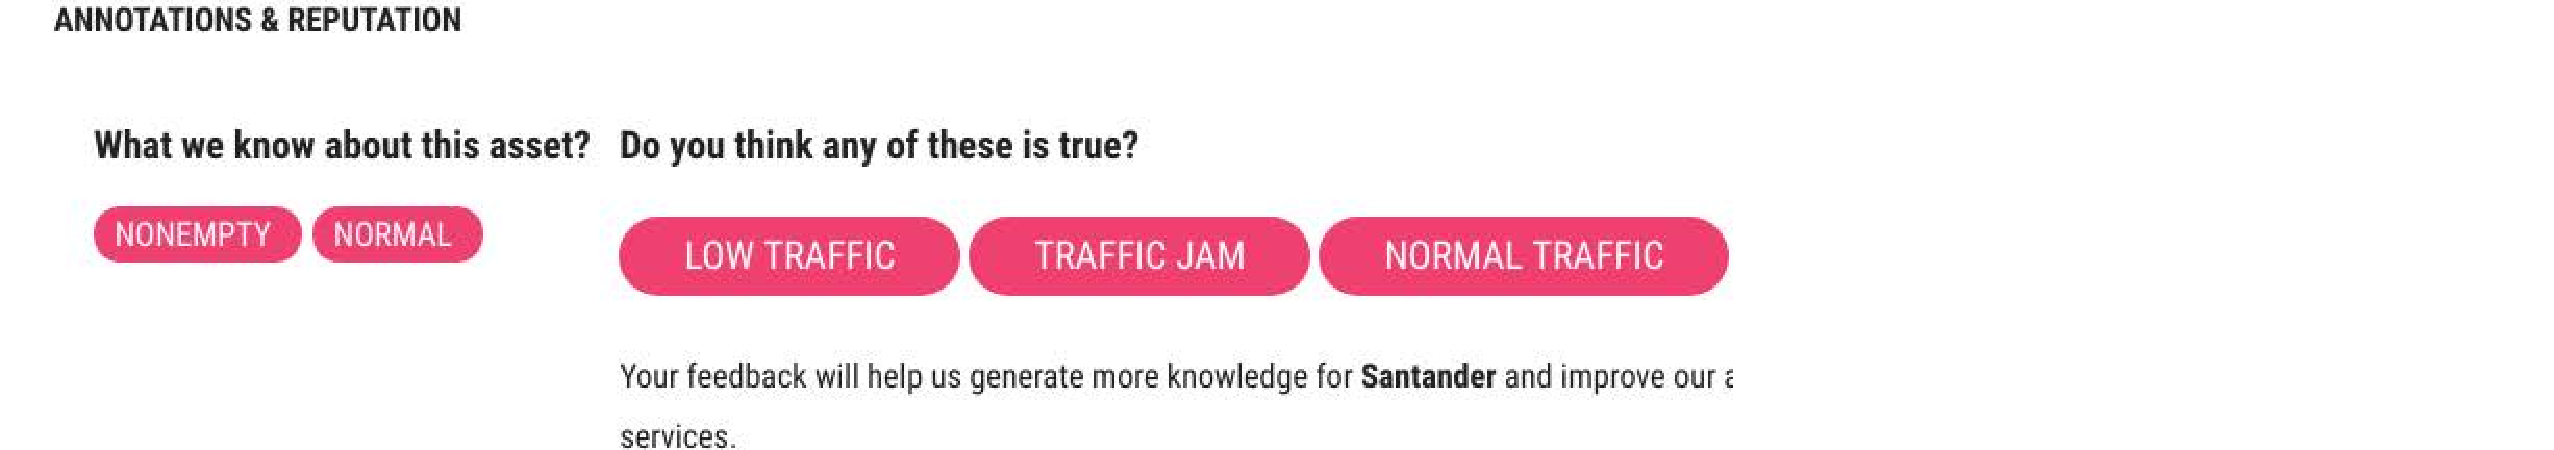
\includegraphics[scale = .3]{figures/annot1}
	\caption{Asset Annotation Interface in the Urban Data Observatory. Asset's annotation (left) and user feedback (right)}
	\label{fig:tags}	
\end{figure}

To further increase the value of the information offered to users, we developed a set of services that operate on top of the generated annotations. % and taxonomies. 
Specifically, we developed a service that automatically adds annotations to the assets of an experiment using Machine Learning (ML), based on provided training datasets. This service allows experimenters to setup and run cloud-based ML jobs to classify the streaming data of the platform in real-time. The process requires a set of initial training data for each of the classifications defined, and the result of the classification is stored as an annotation in the Annotation Service. For each job, the user needs to select a set of tags from the Annotation Service and submit the respective training data. The ML substrate of the system is implemented using JavaML~\cite{abeel2009java}, but is modular in design, i.e., other ML algorithms, e.g., %Apache FlinkML\footnote{https://ci.apache.org/projects/flink/flink-docs-release-1.2/dev/libs/ml/index.html} or 
Google TensorFlow~\cite{abadi2016tensorflow}, can be added in the future.
% based on user requirements.
In its implementation, we use the same principles of the WebSocket Tool and Orion's subscription mechanism to receive real-time updates on the data and trigger the analysis. It creates a subscription for a set of assets the user selects based on URIs and data types to receive updates. Additionally, this service provides a RESTful API so that users can submit external data for classification. If the asset submitted in both cases is available in OC, then the resulting classification is stored in the Annotation Service and propagated to the Orion. If the asset is not available in OC, the classification is simply returned as a response to the API request. More information on the mechanism used to generate the annotations is available in~\cite{Jamaica}.

During the experimentation and the operation of the platform in the past months, users of OC have produced more than 42000 annotations, using over 100 different tags provided either by OC or the experimenters involved.

\subsection{Reputation}

\highlighttext{The \textit{Reputation Service} uses direct and indirect information from the OC platform users, to make it easier to navigate inside the assets available on the OC platform.} It calculates a \emph{reputation} for each asset as a single rating that captures its popularity and usefulness to the end-users. Reputation can also be perceived as trust, by modeling the degree of trust end-users assign to each specific asset. We focus on the generic notion of reputation, that is public and combined, and not a personal/subjective one. 

The Reputation Service is embedded in the UDO and uses statistical data from the Annotation Service.
% presented in \Cref{sec:annotation-service}. 
The reputation score is first calculated after a user has interacted with the assets for the first time. To generate a reputation score, a user has to either create an annotation for the specific asset, or to manually rate it. The rating information is submitted from the UDO to the Annotation Service and triggers an update to the reputation of the asset. When a user selects an asset, the UDO retrieves non-zero reputation statistics from Annotation Service and calculates the reputation score based on a weight-based model. This architecture is more efficient than a stand-alone reputation service, as it removes the requirement for an additional service, and allows for more dynamic values for reputation as they are calculated on request on the user's end. Furthermore, the overhead due to the update and retrieval of the statistics is negligible, as the UDO communicates internally with the Annotation Service with minimal network delays.

For modeling the reputation of assets, we employ a statistical based model due to its simplicity, lightweight computational requirements and the extendibility by easily integrating new parameters when necessary. The reputation model is based on both subjective and objective parameters of the assets:

\begin{itemize}
	\item Opinion represented as a 5-star rating.
	\item Usage of statistics/popularity: How many times an Asset has been annotated by users?
            How many times has an Asset been rated by different users?
	\item Time of the most recent action: What was the last time that an Asset has been annotated?
\end{itemize}	

\highlighttext{The final trust value is calculated as the average of all the parameters}. The interface through which users can add their rating of an asset or view its reputation is presented in \Cref{fig:rep}.

\begin{figure}
	\centering
	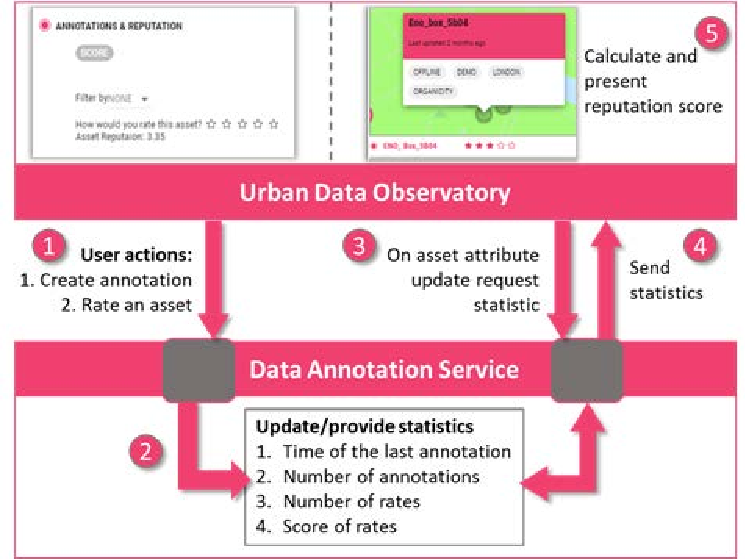
\includegraphics[scale = .65]{figures/repu1}
	\caption{Asset Reputation interface in the Urban Data Observatory (user input and calculated value)}
	\label{fig:rep}	
\end{figure}


